\section{Zielsetzung}

\section{Theorie}

\section{Durchführung}

\section{Auswertung}
\subsection{Entladevorgang eines Kondensators}

\begin{table}
  \centering
  \caption{Messwerte: Entladung eines Kondensators.}
  \label{table1}
  \begin{tabular}{c c}
    \toprule
    $t$ / ms & $U(t)$ / mV \\
    \midrule
    -5.500 & 720\\
    -5.400 & 500\\
    -5.300 & 320\\
    -5.200 & 160\\
    -5.100 & 20\\
    -5.000 & -120\\
    -4.900 & -220\\
    -4.800 & -320\\
    -4.700 & -400\\
    -4.600 & -460\\
    -4.500 & -560\\
    -4.400 & -620\\
    -4.300 & -660\\
    -4.200 & -700\\
    -4.100 & -740\\
    -4.000 & -800\\
    -3.900 & -820\\
    -3.800 & -840\\
    -3.700 & -860\\
    -3.600 & -880\\
    -3.500 & -900\\
    -3.400 & -920\\
    -3.300 & -940\\
    -3.200 & -940\\
    -3.100 & -960\\
    -3.000 & -960\\
    -2.900 & -980\\
    -2.800 & -980\\
    -2.700 & -980\\
    \bottomrule
  \end{tabular}
\end{table}

Bei der ersten Methode zur Bestimmung von $RC$ (Zeitkonstanten) wird der Entladevorgang eines Kondesators
über einen Widerstand beobachtet. Zunächst werden die Werte so im Graphen verschoben, sodass $U(t=0)=U_\symup{max}$
und $U(t \to \infty) = 0$ gilt.

\begin{figure}
  \centering
  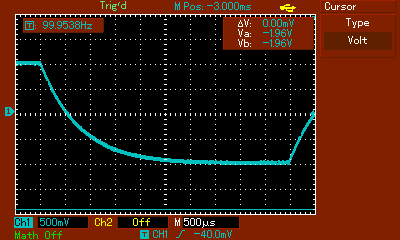
\includegraphics[scale = 0.5]{Bild1.png}
  \caption{Entladevorgang eines Kondensators.}
  \label{Bild1}
\end{figure}

\begin{figure}
  \centering
  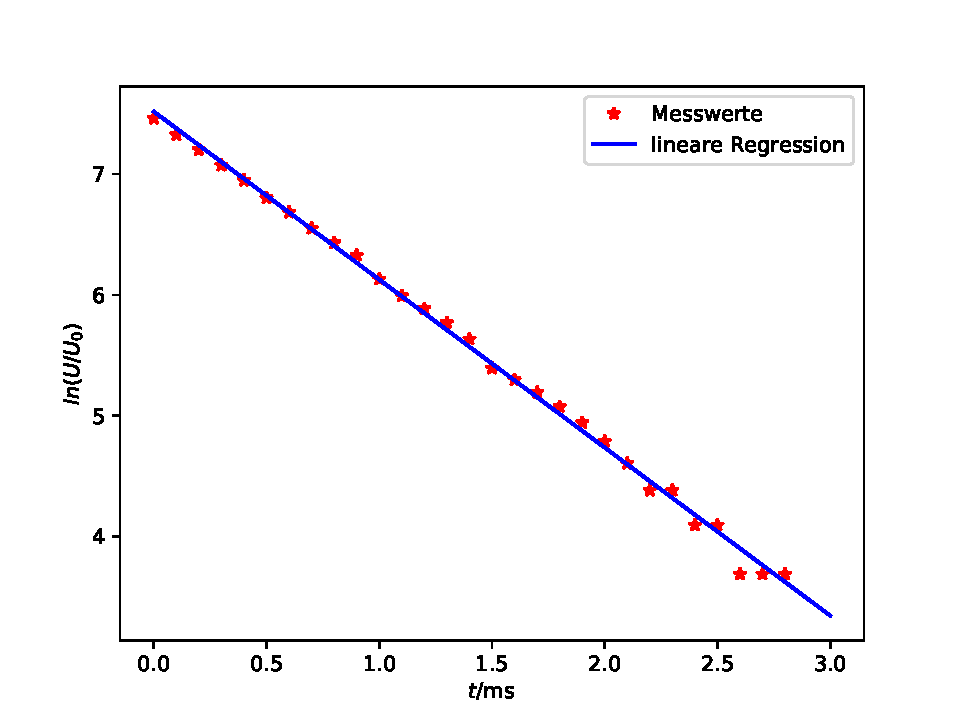
\includegraphics[scale = 0.7]{plotA.pdf}
  \caption{Messwerte und lineare Regression zur Entladung eines Kondensators.}
  \label{PlotA}
\end{figure}

Aus dem Diagramm aus Abbildung \ref{Bild1} werden 30 Wertepaare entnommen,
die Spannngen logarithmiert und in die Abbildung \ref{PlotA} eingetragen. Mit den Wertepaaren wird eine
lineare Regression durchgeführt, wobei die Steigung $m$ und der y-Achsenabschnitt $b$ wie folgt definiert sind:

\begin{align*}
  m &= - \frac{1}{RC} \\
  b &= ln(Q(0))
\end{align*}

wobei $R$ den Widerstand, $C$ die Kapazität des Kondensators, $Q(0)$ die Ladung des Kondensators zum Zeitpunkt
$t=0$ beschreibt. Mit Hilfe der linearen Regression werden die Werte für $m$ und $b$ ermittelt

\begin{align*}
  m &= \SI{-1391(14)}{\per\second} \\
  b &= \SI{0.608(23)}{\ln(C)}.
\end{align*}

Mit

\begin{equation*}
  RC = -\frac{1}{m} \, ,
\end{equation*}

folgt direkt

\begin{equation*}
  RC = \SI{0.719(7)}{\milli\second} \, .
\end{equation*}

\subsection{Frequenzabhängigkeit der Amplitude}

\begin{table}
  \centering
  \caption{Messwerte: Frequenzabhängigkeit der Amplitude.}
  \label{table2}
  \begin{tabular}{c c}
    \toprule
    $\nu$ /Hz & $U$ /mV \\10  940\\
    \midrule
    10 & 940\\
    20 & 960\\
    30 & 980\\
    40 & 960\\
    50 & 940\\
    60 & 940\\
    70 & 920\\
    80 & 900\\
    90 & 880\\
    100 & 860\\
    200 & 700\\
    300 & 540\\
    400 & 432\\
    500 & 360\\
    600 & 312\\
    700 & 272\\
    800 & 240\\
    900 & 216\\
    1000 & 188 \\
    2000 & 96\\
    3000 & 64.4\\
    4000 & 48.8\\
    5000 & 39.2\\
    6000 & 32.8\\
    7000 & 27.6\\
    8000 & 24.0\\
    9000 & 31.6\\
    10000 &  19.2\\
    \bottomrule
  \end{tabular}
\end{table}

Bei der zweiten Methode zur Bestimmung der Zeitkonstanten $RC$ wird die Abhängigkeit der
Amplitude $A(\nu)$ von der Frequenz augenutzt. Die Messwerte werden wieder in ein Diagramm eingetragen
und es wird eine Regression der Form

\begin{equation*}
  \frac{A(\nu)}{U_0} = \frac{1}{\sqrt{1+(2 \pi \nu RC)^2}}
\end{equation*}

durchgeführt, wobei $U_0$ die Amplitude der ungedämpften Schwingung ist.
Die Regression ergibt den Wert der Zeitkonstanten

\begin{equation*}
  RC = \SI{0.771(8)}{\milli\second}.
\end{equation*}

\begin{figure}
  \centering
  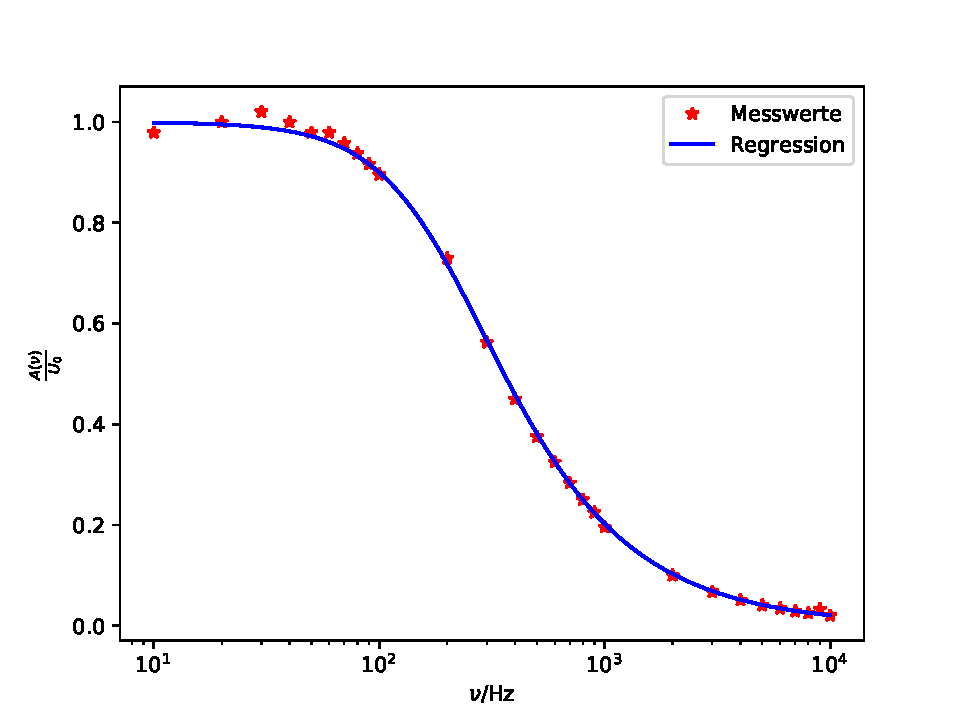
\includegraphics[scale = 0.7]{plotB.pdf}
  \caption{Amplitude $A(\nu)$ in Amhängigkeit der Frequenz $\nu$}
  \label{Plot2}
\end{figure}

\subsection{Frequenzabhängikeit der Phasenverschiebung}

\begin{table}
  \centering
  \caption{Messwerte: Frequenzabhängigkeit der Phasenverschiebung. Wobei $\Delta t$ die Zeitdifferenz
  zwischen der gedämpften und ungedämpften Schwingung und $T$ die Periodendauer einer Schwingung ist.}
  \label{table3}
  \begin{tabular}{c c c}
    \toprule
    $\nu$ / Hz & $\Delta t$ / $\mu$ s & $T$ / ms \\
    \midrule
    10 & 680 & 100\\
    20 & 720 & 50\\
    30 & 740 & 33\\
    40 & 740 & 25\\
    50 & 760 & 20\\
    60 & 740 & 16.72\\
    70 & 724 & 14.32\\
    80 & 708 & 12.4\\
    90 & 700 & 11.2\\
    100 & 684 & 10\\
    200 & 640 & 4.98\\
    300 & 520 & 3.32\\
    400 & 432 & 2.5\\
    500 & 384 & 1.98\\
    600 & 328 & 1.66\\
    700 & 288 & 1.44\\
    800 & 264 & 1.24\\
    900 & 232 & 1.13\\
    1000 & 216 & 0.992\\
    2000 & 116 & 0.500\\
    3000 & 80 & 0.332\\
    4000 & 60 & 0.250\\
    5000 & 47 & 0.200\\
    6000 & 37 & 0.167\\
    7000 & 33 & 0.142\\
    8000 & 33 & 0.125\\
    9000 & 27 & 0.111\\
    10000 & 25 & 0.100\\
    \bottomrule
  \end{tabular}
\end{table}

Zunächst in wird der Phasenunterschied $\Delta\phi$ mit Hilfe der Formel

\begin{equation*}
  \Delta\phi = \frac{\Delta t}{T} \cdot 2 \pi
\end{equation*}

berechnet. Analog zu den Methoden vorher, werden die Werte in ein Diagramm eingetragen und eine
Regression der Form

\begin{equation*}
  \Delta\phi(\nu) = \arctan (-2 \pi \nu RC)
\end{equation*}

durchgeführt. Die Regression liefert den Wert für dei Zeitkonstante

\begin{equation*}
  RC = \SI{0.767(25)}{\milli\second}
\end{equation*}

\begin{figure}
  \centering
  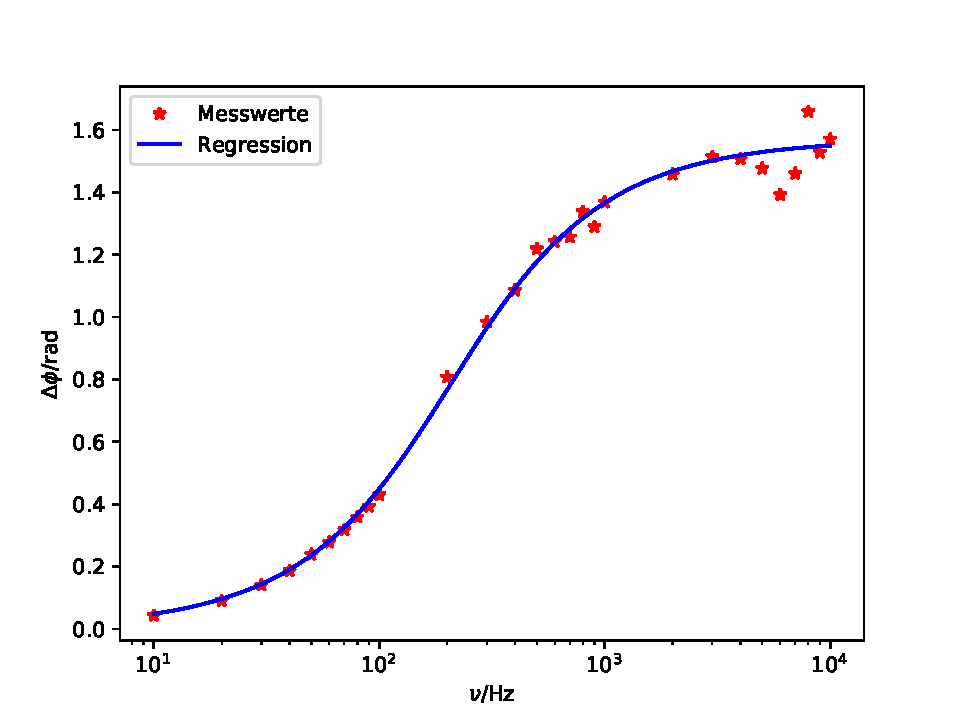
\includegraphics[scale = 0.7]{plotC.pdf}
  \caption{Phasenverschiebung $\Delta\phi (\nu)$ in Abhängigkeit der Frequenz $\nu$}
  \label{Plot3}
\end{figure}

\subsection{RC-Kreis als Integrantor}

Man kann für bestimmte Bedingungen den RC-Kreis auch als Integrantor dienen. Eine Bedingung dafür
ist eine hohe Frequenz, in unserem Versuch werden die Bilder mit einer Frequenz von 100 kHz
aufgenommen. Folgend beschreiben die gelben Funktionen die Ausgangsspannung und die blauen Funktionen
die Spannung über den RC-Kreis.

\begin{figure}[h!]
  \centering
  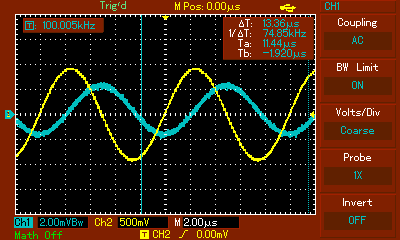
\includegraphics[scale = 0.6]{Bild2.png}
  \caption{RC-Kreis als Integrator, Sinusschwingung.}
  \label{Integrator1}
\end{figure}

\begin{figure}[h!]
  \centering
  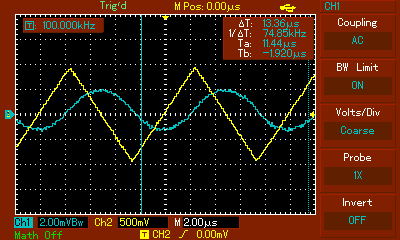
\includegraphics[scale = 0.6]{Bild4.png}
  \caption{RC-Kreis als Integrator, Dreiecksspannung}
  \label{Integrator2}
\end{figure}

\begin{figure}[h!]
  \centering
  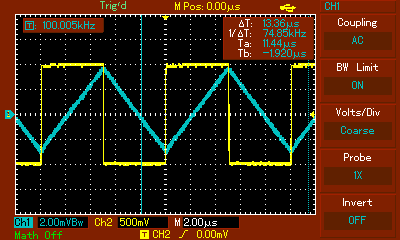
\includegraphics[scale = 0.6]{Bild5.png}
  \caption{RC-Kreis als Integrator, Rechteckschwingung}
  \label{Integrator3}
\end{figure}

In Abbildung \ref{Integrator1} wird eine Sinusspannung durch den Spannungsgenerator erzeugt.
Es lässt sich erkennen, dass die blaue Spannung eine  negative Cosinusfunktion (an der x- Achse gespiegelt) darstellt,
welchemathematisch auch das Integral einer Sinusfunktion ist.

In Abbildung \ref{Integrator2} wird eine Dreiecksspannung erzeugt. Hier lässt sich erkennen, dass die
Integrationsfunktion aus Parabeln besteht. Mathematisch gesehen wird aus einer Geraden nach der Integration
eine Parabel, welches den RC-Kreis aus Integrator bestätigt.

In Abbildung \ref{Integrator3} wird eine Rechteckschwingung angelegt. Mathematisch gesehen, ist
das Integral einer konstanten Funktion eine Geraden, wobei der Wert der Funktion der Steigung entspricht.
Hier ist zu erkennen, dass aus einer Rechteckfunktion nach der Integration eine Dreiecksfunktion wird,
welche aus unendlich vielen Geraden besteht. Auch hier lässt sich die FUnktion des RC-Kreises als
Integrator gut erkennen.

\section{Diskussion}

\begin{table}
  \centering
  \caption{Vergleich der Werte für die Zeitkonstante}
  \label{Vergleich}
  \begin{tabular}{c c c c}
    \toprule
    & Entladung & Amplitude & Phase \\
    \midrule
    $RC$ / ms & \num{0.719(7)} & \num{0.771(8)} & \num{0.767(25)} \\
    \bottomrule
    \end{tabular}
\end{table}

In Tabelle \ref{Vergleich} sind die einzelnen experimentell ermittelten Zeitkonstanten aufgelistet.
Zu erkennen ist, dass alle Zeitkonstanten in der Gleichen Größenordnung liegen. Dennoch gibt es
Abweichung, wobei dort auch systematische Fehler vorhanden sind, denn bei allen Versuchen wird der
Innenwiderstand des Generators vernachlässigt.
Weitere Fehler lassen sich auf Messfehler zurückführen. Diese haben ihren Ursprung beim Errechnen der Werte
des Oszilloskops, da bei größerern Frequenzen die zu messenden Größen immer kleiner werden und das
Oszilloskop beispielsweise bei der Messung der Amplituden nur in 20mV-Schritten messen kann.
